\section{BigchainDB Implementation Details}\label{sec:implementation}

\subsection{Choice of Distributed DB}
The BigchainDB design is flexible enough to have been built on top of a wide variety of existing distributed DBs.
Of course, we had to choose a first one to build on.
To select which, we first did benchmarking, then added additional criteria.

There are $>100$ DBs to choose from, listed for example at \cite{nosql} and \cite{toad2015toad}.
This was our shortlist: Cassandra \cite{cassandra}, HBase \cite{hbase}, Redis \cite{redis}, Riak \cite{riak}, MongoDB \cite{mongodb}, RethinkDB \cite{rethinkdb}, and ElasticSearch \cite{elasticsearch}.
Each of these DBs uses Paxos or a Paxos descendant such as Raft \cite{ongaro2014raft}.

First, we did preliminary performance investigation of the DBs in our shortlist: Each had $15-105$ writes/s per thread, $290-1000$ serial reads/s per thread, and $80-400$ reads/s per thread.

While there was some variation in performance among the DBs, the key thing to notice is that performance is per thread: performance improves as the number of threads increases.
This is different than traditional blockchain technologies, where performance stays flat or worsens.

Given that all DBs tested had good scalability properties, we realized that other criteria were even more important. In particular:
\begin{enumerate}
 \item \textbf{Consistency.} Distributed DBs must make a trade-off between performance and consistency (in the CAP theorem \cite{wiki_cap} sense, not ACID sense \cite{wiki_acid}). For a blockchain, consistency means trustworthy ordering of transactions, so we prefer DBs with strong consistency guarantees.
 \item{\textbf{Automatic Change Notifications.} One way for a node to find out if a change has happened in a DB is to ask it on a regular basis (i.e. polling), but that’s not as efficient as having the DB automatically notify the node of changes.
  We wanted a DB with automatic change notifications as a standard feature.
  
  \medskip
  Automatic change notifications bring another benefit: they improve tamper-resistance (beyond what a chain of hashes offers).
  If a hacker somehow manages to delete or update a record in the data store, the hashes change (like any blockchain).
  In addition, a datastore with automatic change notifications would notify all the nodes, which can then immediately revert the change and restore the hash integrity.}
\end{enumerate}

Of the options considered, we found that RethinkDB met our needs best.
It has strong consistency guarantees \cite{rethinkdb_consistency} and it offers automatic change notifications (“changefeeds”) as a standard feature \cite{rethinkdb_changefeeds}.
Therefore, we built the first version of BigchainDB on top of RethinkDB.

RethinkDB is a JSON (NoSQL) database with a flexible query language \cite{rethinkdb_faq}.
It is optimized for scalable realtime feeds, which is useful for collaborative apps, streaming analytics, multiplayer games, realtime marketplaces, and connected devices / IoT\footnote{IoT = Internet of Things}.
It is written in C++, is open source, and has a vibrant development community \cite{rethinkdb_github}.

In the future, we envision a variety of distributed databases being “blockchain-ified” according to the approach of this paper.
Every relational database, document store and graph store might someday have a blockchain version.


\subsection{BigchainDB Capacity}

Each node in the RethinkDB cluster adds its own storage capacity to the total database capacity.

For example, if each RethinkDB node were run on a d2.8xlarge instance on Amazon Web Services (AWS), then each of those instances could contribute its $(24 \times 2000)$~GB~$= 48000$~GB of storage to the database. 32~nodes would have $32 \times 48000 = 1536000$~GB total capacity, i.e.~more than a petabyte. (This calculation assumes no replication. A replication factor of $R$ would decrease the total capacity by a factor of $R$.)

For quick reference, Figure~\ref{fig:bigchain_capacity_vs_nodes} shows how total capacity depends on the number of nodes. 

\begin{figure}[!ht]
  \centering
  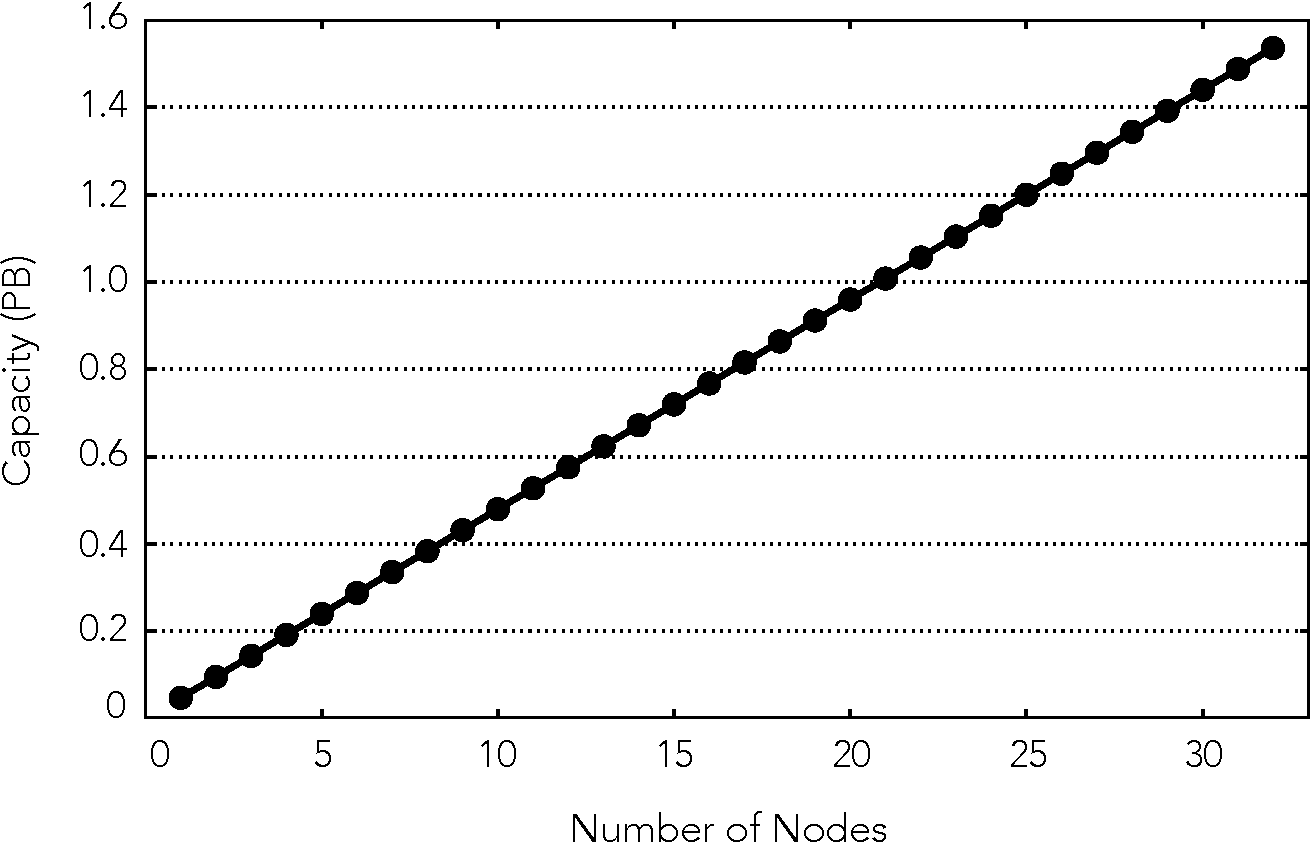
\includegraphics[width=0.8\textwidth]{figure_10.pdf}
  \caption{BigchainDB Capacity versus Number of Nodes. Each node adds another $48000$~GB to the total storage capacity.}
  \label{fig:bigchain_capacity_vs_nodes}
\end{figure}


\subsection{Serialization}

Before we can hash or sign a JSON message (e.g.~a transaction payload), we must convert it to a string in a standard way (i.e.~with the same result, regardless of the programming language or computer architecture used). That is, we must serialize the JSON message in a standard way. Fortunately, there \emph{is} a standard: RFC 7159 \cite{RFC7159}.

We do JSON serialization using the \texttt{dumps()} function in \texttt{python-rapidjson}\footnote{\url{https://github.com/kenrobbins/python-rapidjson}}, a Python wrapper for \texttt{rapidjson}\footnote{\url{https://github.com/miloyip/rapidjson}} (a fast and RFC 7159-compliant JSON parser/generator written in C\nolinebreak[4]\hspace{-.05em}\raisebox{.4ex}{\tiny\bf ++}). Here's how we call it:

\medskip
\begin{minipage}{\linewidth}
  \begin{lstlisting}[style=python]
  import rapidjson 
  rapidjson.dumps(data, 
                  skipkeys=False, 
                  ensure_ascii=False, 
                  sort_keys=True)\end{lstlisting}
\end{minipage}

\medskip
\noindent Here's what the parameters mean: 
\begin{itemize}
 \item $\mathtt{data}$ is the JSON message, stored in a Python dict
 \item $\mathtt{skipkeys = False}$: Ensures that all keys are strings
 \item $\mathtt{ensure\_ascii = False}$: The RFC recommends UTF-8 encoding for maximum interoperability. By setting $\mathtt{ensure\_ascii}$ to $\mathtt{False}$ we allow Unicode characters and force the encoding to UTF-8
 \item $\mathtt{sort\_keys = True}$: The output is sorted by keys
\end{itemize}


\subsection{Cryptography}

This section outlines the cryptographic algorithms used by BigchainDB.

\subsubsection{Cryptographic Hashes}

All hashes are calculated using the SHA3-256 algorithm. We store the hex-encoded hash in BigchainDB. Here is a Python implementation example, using \texttt{pysha3}\footnote{\url{https://bitbucket.org/tiran/pykeccak}}:

\medskip
\begin{minipage}{\linewidth}
  \begin{lstlisting}[style=python]
  import hashlib 
  # monkey patch hashlib with sha3 functions 
  import sha3 
  data = "message" 
  tx_hash = hashlib.sha3_256(data).hexdigest()\end{lstlisting}
\end{minipage}


\subsubsection{Keys and Signatures}

We use the Ed25519 public-key signature system \cite{ed25519} for generating public/private key pairs (also called verifying/signing keys). Ed25519 is an instance of the Edwards-curve Digital Signature Algorithm (EdDSA). As of April 2016, EdDSA was in “Internet-Draft” status with the IETF but was already widely used \cite{I-D.irtf-cfrg-eddsa, ed25519-users}.

BigchainDB uses the the \texttt{ed25519} Python package\footnote{\url{https://github.com/warner/python-ed25519}}, overloaded by the cryptoconditions library\footnote{\url{https://github.com/bigchaindb/cryptoconditions}}.

All keys are represented using base58 encoding by default.
